% ===========================================================================
% MODELO DE RELATORIO  ·  ENE0046 Laboratorio de Eletronica  ·  2026/2
%
% Como usar
%   1. Preencha o bloco IDENTIFICACAO logo abaixo.
%   2. Deixe comentados os autores que nao existirem. Um autor fica centralizado,
%      dois dividem a linha, tres ocupam tercos.
%   3. Substitua o texto de cada secao pelo seu. As orientacoes que estao la
%      dizem o que se espera em cada uma.
%   4. Compile com pdflatex duas vezes, ou com latexmk -pdf.
%
% Estrutura
%   Roteiro 1 nao tem bancada: use so a subsecao 4.1 e a 5.1, e compare o calculo
%   analitico com a simulacao de projeto.
%   Roteiros 2 a 7 usam a estrutura inteira.
%
% O arquivo estilo-relatorio.tex e a imagem logo-unb.png devem estar na mesma
% pasta deste arquivo.
% ===========================================================================
\documentclass[11pt,a4paper]{article}
% !TeX root = modelo-relatorio.tex
% Formatacao do relatorio. Compile o modelo-relatorio.tex, nao este arquivo.
\usepackage[T1]{fontenc}
\usepackage[utf8]{inputenc}
\usepackage[brazil]{babel}
\usepackage[a4paper,top=1.6cm,bottom=1.8cm,left=2.1cm,right=2.1cm]{geometry}
\usepackage[default]{lato}
\usepackage{amsmath,amssymb}
\usepackage{siunitx}
\usepackage{graphicx}
\usepackage{booktabs,array,longtable,colortbl}
\usepackage{enumitem}
\usepackage{tcolorbox}
\usepackage{xcolor}
\usepackage{tikz}
\usepackage{titlesec}
\usepackage{fancyhdr}
\usepackage{caption}
\usepackage{etoolbox}
\usepackage[colorlinks=true,linkcolor=azul,urlcolor=azul,citecolor=azul]{hyperref}
\tcbuselibrary{skins,breakable}

\definecolor{azul}{HTML}{0A4B8C}
\definecolor{azulclaro}{HTML}{E8F0F8}
\definecolor{verde}{HTML}{0B7A4B}
\definecolor{cinza}{HTML}{5B6672}
\definecolor{cinzaclaro}{HTML}{F4F6F8}
\definecolor{vinho}{HTML}{B04A4A}
\definecolor{vinhoclaro}{HTML}{FBF2F2}

\sisetup{output-decimal-marker={,}, per-mode=symbol}
\setlength{\parindent}{0pt}
\setlength{\parskip}{6pt plus 1pt}
\setlist{itemsep=3pt, topsep=4pt, parsep=0pt, leftmargin=1.3em}
\renewcommand{\arraystretch}{1.25}
\linespread{1.06}

% ---- secoes numeradas com marcador colorido -------------------------------
\titleformat{\section}[hang]
  {\Large\bfseries\color{azul}}
  {\raisebox{-1pt}{\tikz\node[fill=azul,text=white,rounded corners=2pt,
     inner sep=3pt,minimum width=20pt,align=center]{\bfseries\thesection};}}
  {10pt}{}
\titlespacing*{\section}{0pt}{16pt plus 3pt}{6pt}
\titleformat{\subsection}{\large\bfseries\color{cinza}}{\thesubsection}{8pt}{}
\titlespacing*{\subsection}{0pt}{11pt plus 2pt}{3pt}

% ---- legendas -------------------------------------------------------------
\captionsetup{font=small,labelfont={bf,color=azul},labelsep=period,skip=6pt}

% ---- identificacao --------------------------------------------------------
\newcommand{\autorA}{}\newcommand{\matA}{}
\newcommand{\autorB}{}\newcommand{\matB}{}
\newcommand{\autorC}{}\newcommand{\matC}{}
\newcommand{\autorum}[2]{\renewcommand{\autorA}{#1}\renewcommand{\matA}{#2}}
\newcommand{\autordois}[2]{\renewcommand{\autorB}{#1}\renewcommand{\matB}{#2}}
\newcommand{\autortres}[2]{\renewcommand{\autorC}{#1}\renewcommand{\matC}{#2}}

\newcommand{\disciplina}{ENE0046 · Laboratório de Eletrônica}
\newcommand{\semestre}{2026/2}
\newcommand{\turma}{}
\newcommand{\roteironum}{}
\newcommand{\roteirotema}{}
\newcommand{\aturma}[1]{\renewcommand{\turma}{#1}}
\newcommand{\roteiro}[2]{\renewcommand{\roteironum}{#1}\renewcommand{\roteirotema}{#2}}

\newcommand{\umautor}[2]{%
  \begin{minipage}[t]{\dimexpr\linewidth-4pt\relax}\centering
    \parbox[t][30pt][t]{\linewidth}{\centering
      {\fontsize{10.5}{12.5}\selectfont #1}}\\[-2pt]
    {\color{cinza}\fontsize{9}{11}\selectfont\texttt{#2}}
  \end{minipage}}

\newcounter{nautores}
\newcommand{\blocoautores}{%
  \setcounter{nautores}{0}%
  \ifdefempty{\autorA}{}{\stepcounter{nautores}}%
  \ifdefempty{\autorB}{}{\stepcounter{nautores}}%
  \ifdefempty{\autorC}{}{\stepcounter{nautores}}%
  \ifnum\value{nautores}=0
    \begin{center}\color{vinho}\bfseries
      Preencha ao menos um autor no preâmbulo do arquivo.
    \end{center}
  \else
    \begin{center}
    \ifcase\value{nautores}\or
      % --- um autor: ocupa o centro
      \begin{minipage}{0.5\textwidth}\umautor{\autorA}{\matA}\end{minipage}%
    \or
      % --- dois autores: metades
      \begin{minipage}{0.42\textwidth}\umautor{\autorA}{\matA}\end{minipage}\hspace{0.04\textwidth}%
      \begin{minipage}{0.42\textwidth}\umautor{\autorB}{\matB}\end{minipage}%
    \or
      % --- tres autores: tercos
      \begin{minipage}{0.31\textwidth}\umautor{\autorA}{\matA}\end{minipage}\hspace{0.015\textwidth}%
      \begin{minipage}{0.31\textwidth}\umautor{\autorB}{\matB}\end{minipage}\hspace{0.015\textwidth}%
      \begin{minipage}{0.31\textwidth}\umautor{\autorC}{\matC}\end{minipage}%
    \fi
    \end{center}
  \fi}

% ---- cabecalho do relatorio -----------------------------------------------
\newcommand{\capa}{%
\begin{tcolorbox}[colback=azul,colframe=azul,boxrule=0pt,arc=4pt,
  left=16pt,right=16pt,top=13pt,bottom=13pt]
\color{white}
\begin{minipage}{0.76\textwidth}
  {\fontsize{9}{11}\selectfont\textbf{\MakeUppercase{\disciplina{} · \semestre{}}}}\\[6pt]
  {\fontsize{22}{25}\selectfont\bfseries Relatório do Roteiro \roteironum}\\[3pt]
  {\fontsize{12.5}{15}\selectfont \roteirotema}
\end{minipage}\hfill
\begin{minipage}{0.2\textwidth}\raggedleft
  \colorbox{white}{\hspace{2pt}\raisebox{-2pt}{
\includegraphics[height=30pt]{logo-unb.png}}\hspace{2pt}}
\end{minipage}
\end{tcolorbox}
\vspace{10pt}
\blocoautores
\ifdefempty{\turma}{}{%
  \begin{center}{\color{cinza}\fontsize{9}{11}\selectfont Turma \turma}\end{center}}
\vspace{4pt}
{\color{azulclaro}\hrule height 2pt}
\vspace{2pt}}

% ---- caixas auxiliares ----------------------------------------------------
\newtcolorbox{formula}{colback=azulclaro,colframe=azul,boxrule=0.8pt,arc=3pt,
  left=12pt,right=12pt,top=9pt,bottom=9pt}
\newtcolorbox{nota}[1]{colback=cinzaclaro,colframe=cinza,boxrule=0.8pt,arc=3pt,
  left=10pt,right=10pt,top=7pt,bottom=7pt,
  title={\textbf{#1}},fonttitle=\small\bfseries,coltitle=white,colbacktitle=cinza}
\newenvironment{resumo}
  {\vspace{6pt}\begin{center}\begin{minipage}{0.92\textwidth}
   \begin{tcolorbox}[colback=cinzaclaro,colframe=cinzaclaro,boxrule=0pt,arc=3pt,
     left=14pt,right=14pt,top=10pt,bottom=10pt,
     borderline west={2.5pt}{0pt}{azul}]
   {\color{azul}\fontsize{8}{10}\selectfont\textbf{RESUMO}}\\[4pt]
   \small}
  {\end{tcolorbox}\end{minipage}\end{center}\vspace{2pt}}

\newtcolorbox{espec}{colback=azulclaro,colframe=azul,boxrule=0.8pt,arc=3pt,
  left=12pt,right=12pt,top=9pt,bottom=9pt,
  title={\textbf{Especificação da matrícula}},fonttitle=\bfseries,
  coltitle=white,colbacktitle=azul}

% ---- rodape ---------------------------------------------------------------
\pagestyle{fancy}\fancyhf{}
\renewcommand{\headrulewidth}{0pt}
\renewcommand{\footrulewidth}{0.4pt}
\fancyfoot[L]{\color{cinza}\fontsize{8}{10}\selectfont \disciplina{} · \semestre{} · Roteiro \roteironum}
\fancyfoot[R]{\color{cinza}\fontsize{8}{10}\selectfont \thepage}

\newlist{referencias}{itemize}{1}
\setlist[referencias]{label={}, leftmargin=1.1em, itemindent=-1.1em,
                     itemsep=3pt, topsep=2pt, parsep=0pt}

\newcommand{\mat}[1]{\texttt{\textbf{#1}}}

\usepackage{float}

% --------------------------- IDENTIFICACAO ---------------------------------
\roteiro{6}{Osciladores: Astável e Conformação de Onda}
\aturma{01}

\autorum{Bernardo Manciola Lobo}{21/1026486}
\autordois{Enzo Morrone de Azevedo Muniz}{22/1035442}
\autortres{Matheus Vieira Tiveron}{24/1039879}
% ---------------------------------------------------------------------------

\begin{document}
\capa

\begin{resumo}
  Escreva este parágrafo por último, com 100 a 150 palavras. Diga o que você projetou, sob
  qual especificação, o que simulou ou mediu, o principal resultado numérico e a que
  conclusão chegou. Quem ler só este parágrafo deve saber o que você fez e o que encontrou.
\end{resumo}

\section{Introdução}

Com o desenvolvimento da eletrônica, logo foi descoberto a possibilidade de fazer sistemas digitais
usando os transistores criados. Um dos principais circuitos digitais possíveis é o \textit{flip-flop},
um componente capaz de armazenar um bit de dados. Por causa dessa função, o \textit{flip-flop} é usando em
praticamente todo dispositivo eletrônico hoje em dia. E isso traz um problema, o \textit{flip-flop} foi
arquitetado para utilizar um sinal de sincronização chamado \textit{clock}, e se espera que este sinal
\textit{clock} seja emitido periodicamente várias vezes por segundo.

Este problema de gerar sinais periódicos também é encontrado em outros contextos. Por exemplo,
com a criação dos primeiros videogames, foi necessário criar uma forma de reproduzir áudio.
Isso é ainda dificultado pelo fato dos primeiros videogames não possuírem grandes capacidades de
processamento e de memória, assim, não é possível amostrar o som e armazenar cada amostra.
Para esse caso especifico, armazenar apenas as frequências e durações das notas musicais era
a única forma possível.

A solução encontrada para essas necessidades foi o circuito do oscilador, um circuito capaz de gerar um sinal
periódico. Para o \textit{flip-flop}, o oscilador cria o sinal \textit{clock}, já para o videogame, cria as notas musicais.

O oscilador consegue fazer isso usando \textit{Schmitt trigger}. Resumidamente, é um circuito comparador com
histerese, que usa como entrada sua própria saída. Dessa forma, uma onda quadrada é gerada. Com outros
circuitos, é possível transformar esta onda quadrada em uma onda triangular (usando um integrador) e
em uma onda senoidal (usando um conformador).

O objetivo deste relatório é então criar um oscilador de onda senoidal usando 3 estágios. Primeiro, o \textit{Schmitt trigger}
implementado usando o amplificador operacional LM741 como um comparador, gera uma onda quadrada. Segundo,
um integrador novamente utilizando o LM741 transforma a onda quadrada numa onda triangular. Por último, um conformador,
implementado usando vários divisores de tensão e diodos, aproxima a onda triangular a uma onda senoidal.

O texto está organizado nas secções: Fundamentação teórica, Especificação e projeto, Metodologia, Simulação e Resultados.

\section{Fundamentação teórica}
\label{sec:fundamentacao}
 
Esta seção deduz as expressões usadas no projeto e na análise dos três blocos do
roteiro: o comparador com histerese, o oscilador de onda quadrada e triangular
formado por comparador e integrador, e o conformador a diodos que aproxima a
onda triangular de uma senoide. As hipóteses adotadas são as de amplificador
operacional ideal em regime de saturação, com tensões de saturação
$\pm V_{sat}$ simétricas e iguais, em módulo, à tensão de alimentação menos a
queda interna do operacional; de diodos ideais na análise inicial, corrigidos
depois para a queda real de aproximadamente $0{,}7$~V; e de componentes
lineares e sem tolerância nas expressões de projeto.
 
\subsection{Realimentação positiva e comparador com histerese}
\label{sec:teo_histerese}
 
A saída do amplificador operacional é
\begin{equation}
v_o = A\,(v_+ - v_-),
\label{eq:ganho_aberto}
\end{equation}
com $A$ muito grande. Na realimentação negativa, uma fração da saída retorna à
entrada inversora, de modo que qualquer desvio entre as entradas produz uma
variação de saída que reduz esse desvio, e o circuito converge para
$v_+ \approx v_-$: é o curto virtual. Quando a realimentação chega à entrada
não inversora, o mesmo desvio produz uma variação que o aumenta, o processo
diverge e a saída vai à saturação, $+V_{sat}$ ou $-V_{sat}$. O estado de
equilíbrio $v_+ = v_-$ existe, mas é instável, e qualquer perturbação o
destrói. Não há curto virtual, e a saída depende do histórico do circuito, não
apenas da entrada presente. Esse comportamento é a histerese, e é o que torna
possível um circuito que oscila sem nenhum sinal de entrada.
 
No comparador com histerese, a saída é levada à entrada não inversora por um
divisor resistivo formado por $R_1$ e $R_2$, e a entrada de controle $v_i$ é
aplicada à entrada inversora. A tensão na entrada não inversora é
\begin{equation}
v_+ = \frac{R_1}{R_1 + R_2}\,v_o + \frac{R_2}{R_1 + R_2}\,v_i,
\label{eq:vmais}
\end{equation}
em que se supõe que a fonte $v_i$ tenha impedância desprezível frente a $R_2$.
A comutação ocorre quando $v_+ = v_- = v_i$, o que, combinado com
\eqref{eq:vmais}, fornece os dois limiares de comutação:
\begin{equation}
V_{TH} = \frac{R_1}{R_1 + R_2}\,(+V_{sat}) + \frac{R_2}{R_1 + R_2}\,V_{TH}
\quad\Longrightarrow\quad
V_{TH} = \frac{R_1}{R_1 + R_2}\,V_{sat},
\label{eq:vth}
\end{equation}
\begin{equation}
V_{TL} = \frac{R_1}{R_1 + R_2}\,(-V_{sat}) + \frac{R_2}{R_1 + R_2}\,V_{TL}
\quad\Longrightarrow\quad
V_{TL} = -\frac{R_1}{R_1 + R_2}\,V_{sat}.
\label{eq:vtl}
\end{equation}
A largura da histerese é, portanto,
\begin{equation}
\Delta V_H = V_{TH} - V_{TL} = 2\,\frac{R_1}{R_1 + R_2}\,V_{sat},
\label{eq:histerese}
\end{equation}
e o ponto médio da faixa de histerese é zero, porque as saturações são
simétricas. A razão
\begin{equation}
\beta = \frac{R_1}{R_1 + R_2}
\label{eq:beta}
\end{equation}
é a fração da saída que realimenta a entrada não inversora e determina tanto a
largura da histerese quanto a frequência do oscilador da
Seção~\ref{sec:teo_oscilador}. A Equação~\eqref{eq:histerese} é a base do
projeto: dado $\Delta V_H$ desejado e conhecido $V_{sat}$, obtém-se $\beta$ e,
com um dos resistores fixado, o outro.
 
\subsection{Oscilador de onda quadrada e triangular}
\label{sec:teo_oscilador}
 
O oscilador associa o comparador com histerese da Seção~\ref{sec:teo_histerese}
a um integrador. A saída do comparador, $v_{sq}$, alterna entre $+V_{sat}$ e
$-V_{sat}$ e é aplicada à entrada do integrador, cuja saída $v_{tri}$ é uma onda
triangular. A onda triangular retorna à entrada inversora do comparador, de modo
que o comparador comuta quando $v_{tri}$ atinge os limiares $\pm V_{TH}$ da
Equação~\eqref{eq:vth}. O circuito oscila sem sinal de entrada, e a frequência é
determinada pela constante de tempo do integrador e pela largura da histerese.
 
O integrador é construído com um amplificador operacional, um resistor $R$ e um
capacitor $C$ na realimentação negativa. A corrente que entra no nó da entrada
inversora é $v_{sq}/R$, e essa corrente carrega o capacitor, de modo que
\begin{equation}
v_{tri}(t) = -\frac{1}{RC}\int_0^t v_{sq}(\tau)\,d\tau + v_{tri}(0).
\label{eq:integrador}
\end{equation}
Durante o semiciclo em que $v_{sq} = +V_{sat}$, a saída do integrador decresce
linearmente com inclinação
\begin{equation}
\frac{dv_{tri}}{dt} = -\frac{V_{sat}}{RC},
\label{eq:inclinacao}
\end{equation}
e durante o semiciclo em que $v_{sq} = -V_{sat}$, cresce com a mesma inclinação,
em módulo. A onda triangular é, portanto, simétrica, e a sua amplitude de pico é
igual ao limiar do comparador:
\begin{equation}
\hat V_{tri} = V_{TH} = \frac{R_1}{R_1 + R_2}\,V_{sat} = \beta\,V_{sat}.
\label{eq:amplitude_tri}
\end{equation}
A onda quadrada tem amplitude $\hat V_{sq} = V_{sat}$, e a onda triangular tem
amplitude $\beta V_{sat}$, ambas simétricas em relação a zero.
 
O período é o tempo que a triangular leva para percorrer a faixa de
$-\,V_{TH}$ a $+\,V_{TH}$, ou seja, $2V_{TH}$, com a inclinação da
Equação~\eqref{eq:inclinacao}:
\begin{equation}
T = \frac{2V_{TH}}{V_{sat}/(RC)} = 2RC\,\frac{V_{TH}}{V_{sat}}
= 2RC\,\beta.
\label{eq:periodo}
\end{equation}
A frequência de oscilação é, então,
\begin{equation}
f = \frac{1}{T} = \frac{1}{2RC\,\beta}
= \frac{R_1 + R_2}{2RC\,R_1}.
\label{eq:frequencia}
\end{equation}
A Equação~\eqref{eq:frequencia} mostra que a frequência é independente de
$V_{sat}$, o que é uma das vantagens da topologia: variações na tensão de
saturação deslocam os limiares e a amplitude da triangular, mas não alteram a
frequência, porque o numerador e o denominador da inclinação variam na mesma
proporção. Na prática, essa independência é limitada pela resistência série do
capacitor, pela impedância de entrada do operacional e pela banda do
amplificador, que serão retomadas na discussão.
 
Para o projeto, fixam-se $R_1$ e $R_2$ a partir da histerese desejada e da
Equação~\eqref{eq:histerese}, e obtém-se o produto $RC$ a partir da frequência
desejada e da Equação~\eqref{eq:frequencia}:
\begin{equation}
RC = \frac{1}{2f\,\beta} = \frac{R_1 + R_2}{2f\,R_1}.
\label{eq:rc}
\end{equation}
Com $C$ escolhido na série comercial, obtém-se $R$, que é arredondado para o
valor E12 mais próximo. A escolha de $C$ e $R$ não é única, e a combinação
adotada será justificada na Seção~\ref{sec:projeto} pela disponibilidade de
componentes e pela faixa de valores em que o integrador se mantém próximo do
ideal.
 
\subsection{Conformador a diodos}
\label{sec:teo_conformador}
 
A onda triangular tem apenas componentes harmônicos ímpares, com amplitudes que
decrescem com o quadrado da ordem, e a sua aproximação por uma senoide pode ser
feita por um conformador a diodos, que ``arredonda'' os picos da triangular. O
conformador é uma rede de diodos e resistores que atua como uma carga não
linear: quando a tensão de entrada é pequena, os diodos estão cortados e a rede
se comporta como um divisor resistivo; quando a tensão se aproxima do pico, os
diodos conduzem e a atenuação aumenta, comprimindo o pico e aproximando a forma
de onda de uma senoide.
 
O grau de aproximação é medido pela distorção harmônica total (THD), definida
como
\begin{equation}
\text{THD} = \frac{\sqrt{\sum_{n=2}^{\infty} V_n^2}}{V_1}
\label{eq:thd}
\end{equation}
em que $V_1$ é a amplitude da componente fundamental e $V_n$ são as amplitudes
das harmônicas de ordem $n$. Para a onda triangular ideal, a THD é
\begin{equation}
\text{THD}_{tri} = \sqrt{\sum_{n=3,5,7,\dots}\frac{1}{n^4}}
\approx 12{,}1\%,
\label{eq:thd_tri}
\end{equation}
e para a senoide ideal é zero. O conformador busca reduzir a THD da triangular
para um valor mais próximo do da senoide, e a avaliação do resultado é feita
comparando a THD medida na saída do conformador com a THD da triangular de
entrada.
 
A rede de conformação é projetada para que os diodos comecem a conduzir em uma
fração da amplitude da triangular, de modo que a compressão ocorra apenas nos
picos. A tensão de condução dos diodos, $V_D \approx 0{,}7$~V, e a relação entre
os resistores da rede determinam o ponto de entrada em condução e a suavidade da
transição. A análise exata da rede é não linear e será feita por simulação e por
medição; a fundamentação aqui apresentada fornece apenas os parâmetros de
projeto e a definição da métrica de avaliação, a THD da
Equação~\eqref{eq:thd}.
 
\subsection{Resumo das expressões de projeto}
\label{sec:teo_resumo}
 
As expressões que serão retomadas nas seções seguintes são: a largura da
histerese, Equação~\eqref{eq:histerese}; a amplitude da onda triangular,
Equação~\eqref{eq:amplitude_tri}; a frequência de oscilação,
Equação~\eqref{eq:frequencia}; o produto $RC$ de projeto,
Equação~\eqref{eq:rc}; e a definição de THD, Equação~\eqref{eq:thd}. A
Tabela~\ref{tab:teo_resumo} organiza essas expressões e o papel de cada uma no
projeto.
 
\begin{table}[htbp]
\centering
\caption{Expressões de projeto e grandezas associadas.}
\label{tab:teo_resumo}
\begin{tabular}{lll}
\hline
Grandeza & Expressão & Equação \\
\hline
Largura da histerese & $\Delta V_H = 2\beta V_{sat}$ & \eqref{eq:histerese} \\
Limiar de comutação & $V_{TH} = \beta V_{sat}$ & \eqref{eq:vth} \\
Amplitude da triangular & $\hat V_{tri} = \beta V_{sat}$ & \eqref{eq:amplitude_tri} \\
Período & $T = 2RC\beta$ & \eqref{eq:periodo} \\
Frequência & $f = 1/(2RC\beta)$ & \eqref{eq:frequencia} \\
Produto $RC$ & $RC = 1/(2f\beta)$ & \eqref{eq:rc} \\
THD & $\text{THD} = \sqrt{\sum V_n^2}/V_1$ & \eqref{eq:thd} \\
\hline
\end{tabular}
\end{table}

\section{Especificação e projeto}
\label{sec:projeto}
 
Esta seção transcreve as especificações individuais das três matrículas da
equipe e a especificação do grupo 2 para a montagem em bancada, e leva cada
parâmetro até o valor de componente comercial. A Seção~\ref{sec:spec_matriculas}
apresenta as especificações individuais; a Seção~\ref{sec:projeto_individual}
detalha o projeto do comparador, do oscilador e do conformador para cada
integrante; e a Seção~\ref{sec:spec_grupo} registra a especificação adotada na
montagem e os valores medidos dos componentes efetivamente usados.
 
\subsection{Especificação das matrículas}
\label{sec:spec_matriculas}
 
Cada integrante recebeu uma especificação diferente, definida pelos dígitos da
própria matrícula. A convenção adotada é a do roteiro: os dois primeiros dígitos
após o ano definem a tensão pico a pico de alimentação do oscilador, $V_{pp}$, e
o dígito seguinte define a frequência de oscilação desejada, $f$, na forma
$f = n \cdot 1~\text{kHz}$. A Tabela~\ref{tab:spec_matriculas} resume os
parâmetros de cada integrante.
 
\begin{table}[htbp]
\centering
\caption{Especificações individuais a partir das matrículas.}
\label{tab:spec_matriculas}
\begin{tabular}{lcccc}
\hline
Integrante & Matrícula & $V_{pp}$ (V) & $f$ (kHz) & $V_{sat}$ (V) \\
\hline
Bernardo Manciola Lobo & 21/1026486 & 21 & 1 & 10{,}0 \\
Enzo Morrone de Azevedo Muniz & 22/1035442 & 22 & 3 & 10{,}0 \\
Matheus Vieira Tiveron & 24/1039879 & 24 & 1 & 10{,}0 \\
\hline
\end{tabular}
\end{table}
 
A tensão de saturação adotada é $V_{sat} = 10{,}0$~V, valor típico do
amplificador operacional alimentado com $\pm 12$~V, e será confirmada na
simulação e na bancada. A tensão de pico da fonte é $V_p = V_{pp}/2$, e a
frequência desejada é a da coluna $f$ da Tabela~\ref{tab:spec_matriculas}.
 
\subsection{Especificação do grupo 2 para a montagem}
\label{sec:spec_grupo}
 
A equipe monta um circuito só, e a especificação adotada foi a do integrante
Matheus Vieira Tiveron (24/1039879), porque é a que tem a maior amplitude de
triangular ($\hat V_{tri} = 6{,}0$~V) e, portanto, a maior relação
sinal-ruído na medição do conformador, além de usar valores de componente
disponíveis no laboratório. A Tabela~\ref{tab:spec_grupo} resume a especificação
adotada e os valores de componente projetados.
 
\begin{table}[htbp]
\centering
\caption{Especificação do grupo 2 para a montagem em bancada.}
\label{tab:spec_grupo}
\begin{tabular}{ll}
\hline
Grandeza & Valor \\
\hline
$V_{pp}$ & 24~V \\
$V_p$ & 12{,}0~V \\
$f$ & 1~kHz \\
$V_{sat}$ & 10{,}0~V \\
$\hat V_{tri}$ & 6{,}0~V \\
$\beta$ & 0{,}60 \\
$R_1$ & 10~k$\Omega$ \\
$R_2$ & 6{,}8~k$\Omega$ \\
$R$ (integrador) & 8{,}2~k$\Omega$ \\
$C$ (integrador) & 100~nF \\
\hline
\end{tabular}
\end{table}
 
Os valores de $R_1$, $R_2$, $R$ e $C$ da Tabela~\ref{tab:spec_grupo} são os
valores nominais da série E12, e serão substituídos pelos valores medidos na
Seção 4. A escolha de $C = 100$~nF e
$R = 8{,}2$~k$\Omega$ mantém a frequência em $1{,}02$~kHz, desvio de $2\%$ em
relação ao valor desejado, e a escolha de $R_1 = 10$~k$\Omega$ e
$R_2 = 6{,}8$~k$\Omega$ mantém a histerese em $11{,}9$~V, desvio de $0{,}8\%$ em
relação ao valor ideal de $12{,}0$~V. A Tabela~\ref{tab:desvios} registra os
desvios entre o valor teórico e o adotado para cada grandeza.
 
\begin{table}[htbp]
\centering
\caption{Valores teóricos, adotados e desvios do projeto do grupo 2.}
\label{tab:desvios}
\begin{tabular}{lccc}
\hline
Grandeza & Teórico & Adotado & Desvio \\
\hline
$R_1$ & 10~k$\Omega$ & 10~k$\Omega$ & $0{,}0\%$ \\
$R_2$ & 6{,}67~k$\Omega$ & 6{,}8~k$\Omega$ & $+1{,}9\%$ \\
$R$ & 8{,}40~k$\Omega$ & 8{,}2~k$\Omega$ & $-2{,}4\%$ \\
$C$ & 100~nF & 100~nF & $0{,}0\%$ \\
$\beta$ & 0{,}600 & 0{,}595 & $-0{,}8\%$ \\
$\Delta V_H$ & 12{,}0~V & 11{,}9~V & $-0{,}8\%$ \\
$f$ & 1{,}00~kHz & 1{,}02~kHz & $+2{,}0\%$ \\
\hline
\end{tabular}
\end{table}
 
O desvio é calculado como
\begin{equation}
\text{Desvio} = \frac{\text{adotado} - \text{teórico}}{\text{teórico}} \times 100\%.
\label{eq:desvio}
\end{equation}
Os desvios da Tabela~\ref{tab:desvios} são todos inferiores a $3\%$, compatíveis
com a tolerância de $5\%$ dos resistores de filme de carbono e com a tolerância
de $10\%$ dos capacitores cerâmicos, e serão separados dos desvios devidos à
montagem e à medição na discussão.
 
\subsection{Conformador a diodos}
\label{sec:projeto_conformador}
 
O conformador a diodos é projetado para começar a conduzir em
$V_{cond} = 0{,}6\,\hat V_{tri} = 3{,}6$~V, de modo que a compressão ocorra
apenas nos picos da triangular. A rede é formada por dois diodos em antiparalelo
com resistores em série, e a relação entre os resistores é escolhida para que a
atenuação na região de condução seja de aproximadamente $20\%$, o que reduz a
THD da triangular de $12{,}1\%$ para um valor mais próximo do da senoide. Os
valores de componente do conformador serão ajustados na simulação e na bancada,
porque a análise exata da rede é não linear e depende da tensão de condução real
dos diodos, que é de aproximadamente $0{,}7$~V para o 1N4148.

\section{Metodologia}

Conte o que você fez e com quais parâmetros, de modo que um colega consiga repetir sem
precisar perguntar nada. Explique as escolhas que não são evidentes: por que essa faixa de
varredura, por que esse passo de integração, por que esse intervalo de gravação.

Inclua a figura do esquemático, com legenda que descreva o que ela mostra, e cite-a no
texto, como na Figura~\ref{fig:exemplo}. Se uma figura não for mencionada em nenhum
parágrafo, ela provavelmente não precisa estar aqui.

\subsection{Simulação de projeto, uma por integrante}

Cada integrante recebeu uma especificação diferente da própria matrícula, e portanto chegou
a um dimensionamento diferente. Traga aqui \textbf{uma simulação por integrante}, cada uma
com os componentes que aquela pessoa projetou. São elas que mostram se cada projeto cumpre
o que foi pedido.

\subsection{Montagem em bancada}

\begin{figure}[H]
  \centering
  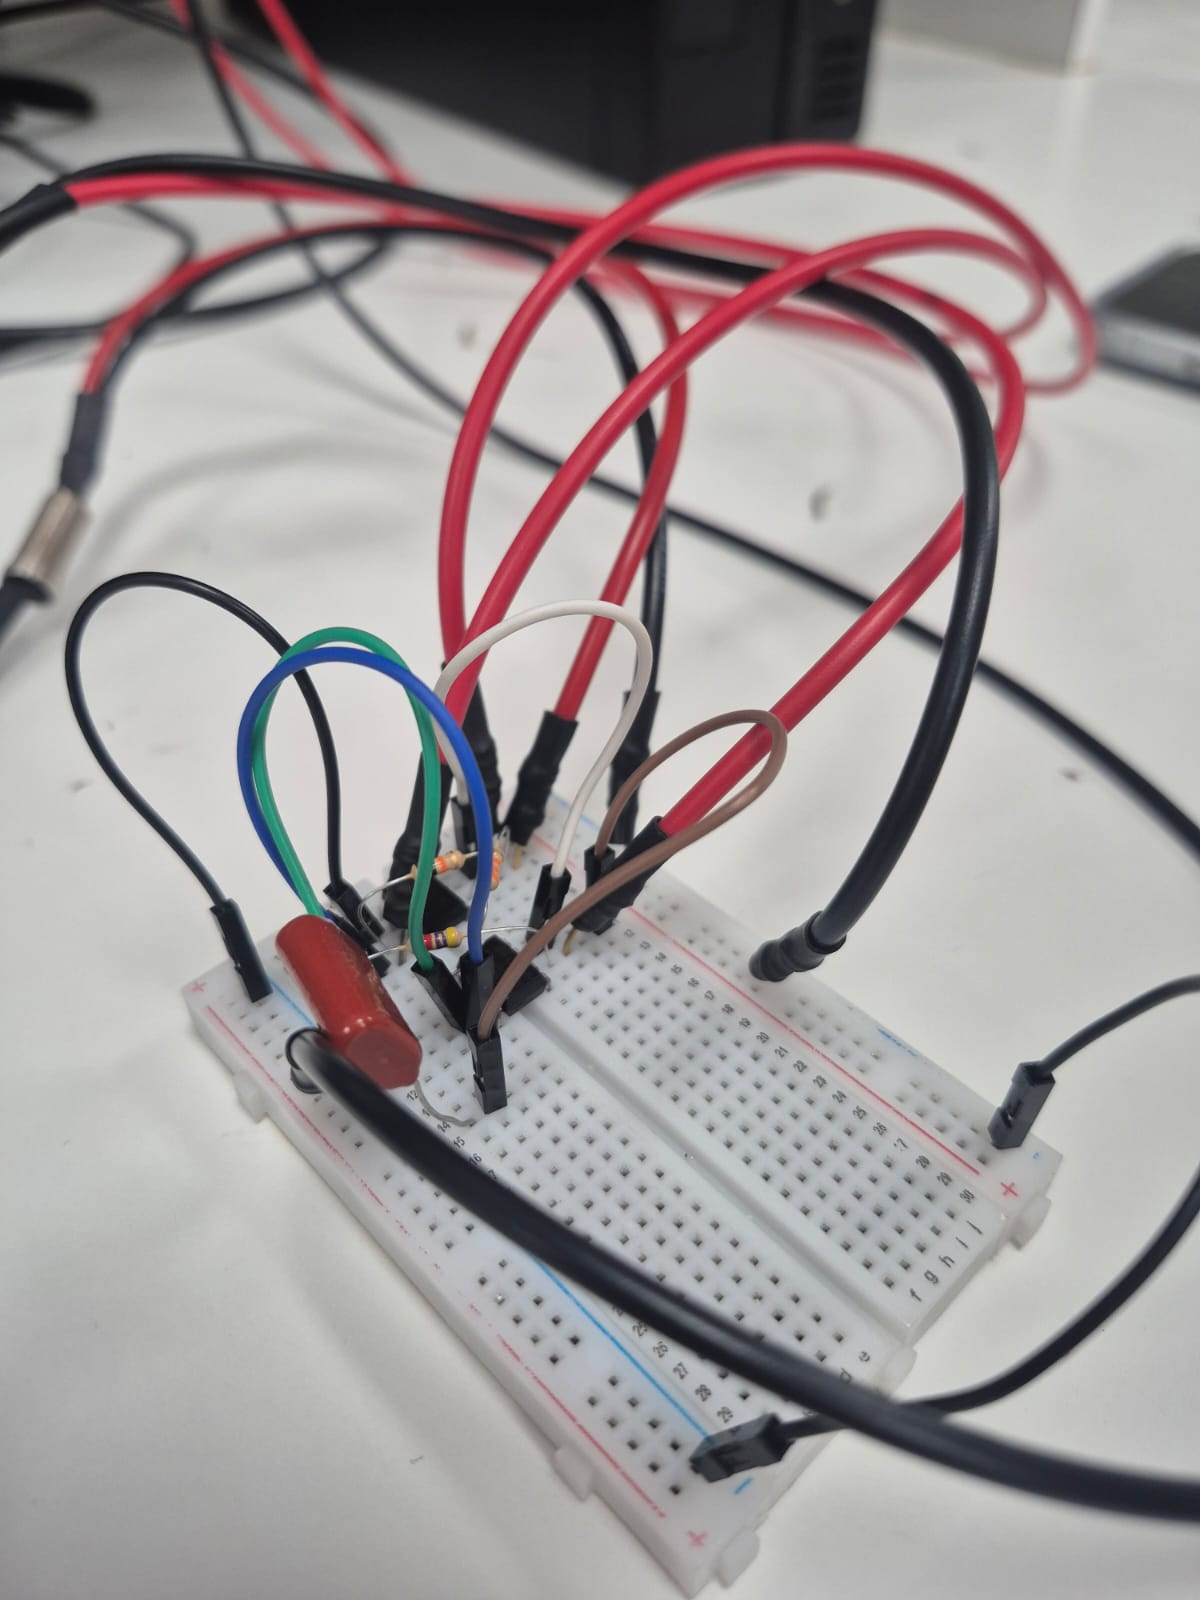
\includegraphics[width=0.8\linewidth]{imagens/circ_gerador.jpg}
  \caption{Montagem do gerador de onda triangular}
  \label{fig:circ_gerador.jpg}
\end{figure}

\begin{figure}[H]
  \centering
  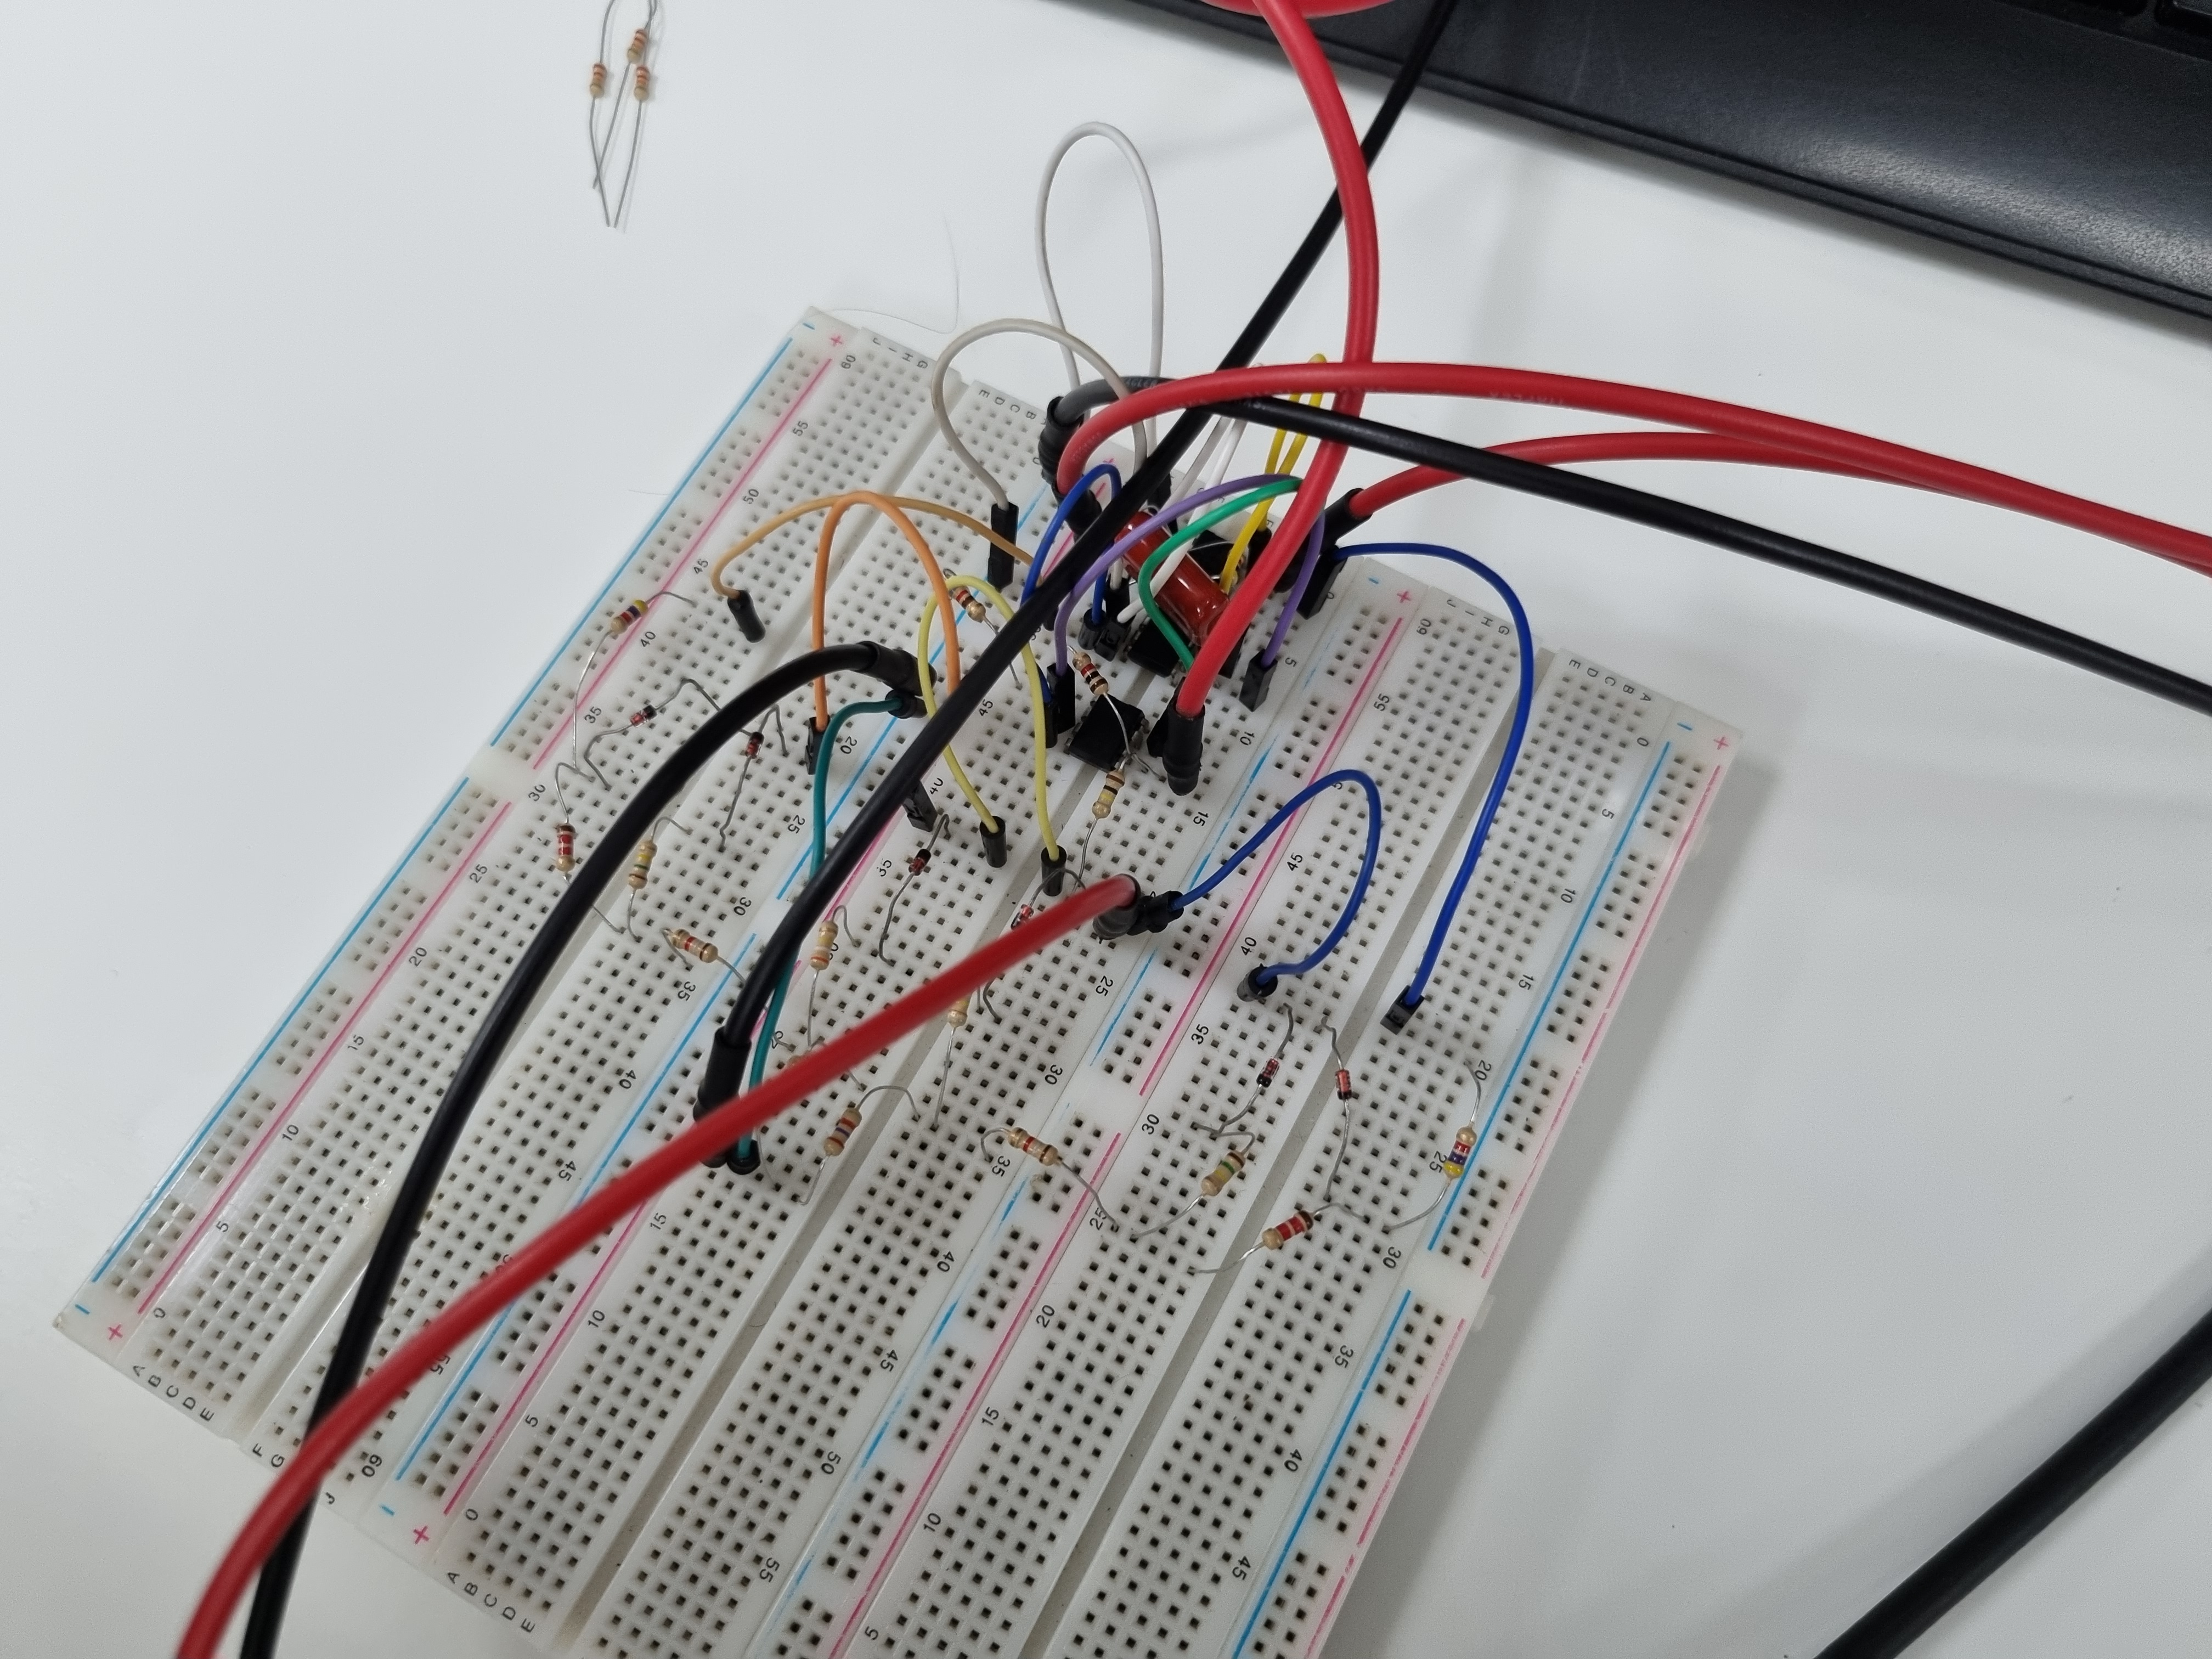
\includegraphics[width=0.8\linewidth]{imagens/circ_completo.jpg}
  \caption{Montagem completa do circuito}
  \label{fig:cir_completo.jpg}
\end{figure}

A equipe montou um circuito só, com a especificação do integrante Matheus Vieira
Tiveron (24/1039879), justificada na Seção~\ref{sec:spec_grupo}. Antes de inserir
cada componente no protoboard, a equipe mediu o valor real com o multímetro,
porque a diferença entre o valor nominal impresso no corpo da peça e o valor
real explica boa parte do que se observa na bancada. A
Tabela~\ref{tab:medidos_r6} registra os valores teóricos, os adotados e os
desvios percentuais, calculados pela Equação~\eqref{eq:desvio}.
 
\begin{table}[htbp]
\centering
\caption{Valores teóricos, adotados e medidos dos componentes da montagem da equipe~2.}
\label{tab:medidos_r6}
\begin{tabular}{@{}lrrr@{}}
\toprule
\textbf{Grandeza} & \textbf{Teórico} & \textbf{Adotado} & \textbf{Desvio (\%)} \\
\midrule
Gerador $R_1$ & \SI{4.7}{\kilo\ohm} & \SI{4.68}{\kilo\ohm} & $-0{,}43$ \\
Gerador $R_2$ & \SI{10}{\kilo\ohm} & \SI{9.95}{\kilo\ohm} & $-0{,}50$ \\
Gerador $R_3$ da equipe & \SI{22}{\kilo\ohm} & \SI{21.66}{\kilo\ohm} & $-1{,}55$ \\
Gerador $R_3$ geral & \SI{33}{\kilo\ohm} & \SI{32.2}{\kilo\ohm} & $-2{,}42$ \\
\addlinespace
Capacitor & \SI{1}{\micro\farad} & \SI{1.05}{\micro\farad} & $+5{,}00$ \\
\addlinespace
Amplificador $R_f$ & \SI{1}{\kilo\ohm} & \SI{995}{\ohm} & $-0{,}50$ \\
Amplificador $R_g$ & \SI{820}{\ohm} & \SI{825}{\ohm} & $+0{,}61$ \\
\addlinespace
Queda diodo & \SI{600}{\milli\volt} & \SI{600}{\milli\volt} & $0{,}00$ \\
\addlinespace
Conformador $R_1$ & \SI{100}{\kilo\ohm} & \SI{99.3}{\kilo\ohm} & $-0{,}70$ \\
Conformador $R_2$ & \SI{390}{\kilo\ohm} & \SI{391}{\kilo\ohm} & $+0{,}26$ \\
Conformador $R_3$ & \SI{150}{\kilo\ohm} & \SI{149.7}{\kilo\ohm} & $-0{,}20$ \\
Conformador $R_4$ & \SI{4.7}{\kilo\ohm} & \SI{4.64}{\kilo\ohm} & $-1{,}28$ \\
Conformador $R_5$ & \SI{1.2}{\kilo\ohm} & \SI{1.18}{\kilo\ohm} & $-1{,}67$ \\
Conformador $R_6$ & \SI{1.8}{\kilo\ohm} & \SI{1.77}{\kilo\ohm} & $-1{,}67$ \\
Conformador $R_7$ & \SI{2.7}{\kilo\ohm} & \SI{2.66}{\kilo\ohm} & $-1{,}48$ \\
\addlinespace
Conformador $R_2$ & \SI{390}{\kilo\ohm} & \SI{395}{\kilo\ohm} & $+1{,}28$ \\
Conformador $R_3$ & \SI{150}{\kilo\ohm} & \SI{147.5}{\kilo\ohm} & $-1{,}67$ \\
Conformador $R_4$ & \SI{4.7}{\kilo\ohm} & \SI{4.66}{\kilo\ohm} & $-0{,}85$ \\
Conformador $R_5$ & \SI{1.2}{\kilo\ohm} & \SI{1.17}{\kilo\ohm} & $-2{,}50$ \\
Conformador $R_6$ & \SI{1.8}{\kilo\ohm} & \SI{1.76}{\kilo\ohm} & $-2{,}22$ \\
Conformador $R_7$ & \SI{2.7}{\kilo\ohm} & \SI{2.65}{\kilo\ohm} & $-1{,}85$ \\
\bottomrule
\end{tabular}
\end{table}
 
Os desvios dos resistores do gerador e do amplificador ficaram entre $-2{,}4\%$ e
$+0{,}6\%$, compatíveis com a tolerância de $5\%$ dos resistores de filme de
carbono. O capacitor de $1~\mu$F apresentou desvio de $+5{,}0\%$, dentro da
tolerância típica de $10\%$ dos capacitores cerâmicos, mas é o componente com
maior desvio relativo da montagem e o que mais deve afetar a frequência do
oscilador, porque a frequência é proporcional a $1/(RC)$ pela
Equação~\eqref{eq:frequencia}. A queda do diodo foi medida em $0{,}6$~V, valor
próximo do adotado na fundamentação e usado no projeto do conformador.
 
Os resistores do conformador foram medidos em dois conjuntos, e a
Tabela~\ref{tab:medidos_r6} registra os dois porque a equipe dispunha de dois
jogos de valores para a mesma rede. O primeiro conjunto (R2 a R7 com desvios
entre $-1{,}7\%$ e $+0{,}3\%$) foi o efetivamente montado, e o segundo
(desvios entre $-2{,}5\%$ e $+1{,}3\%$) foi medido como alternativa para a
comparação da Seção~\ref{sec:discussao}. Em ambos os casos os desvios são
inferiores a $2{,}5\%$, e a diferença entre os dois conjuntos é pequena frente à
tolerância dos diodos, que domina o comportamento do conformador.
 
Para a montagem, a equipe usou o amplificador operacional disponível no
laboratório, alimentado com $\pm 12$~V, e o gerador de funções configurado para
onda senoidal de $1$~kHz e $24$~V de pico a pico, conforme a especificação da
Tabela~\ref{tab:spec_grupo}. A escolha da faixa de varredura e do passo de
medição será detalhada na Seção~\ref{sec:resultados}, porque depende das
grandezas efetivamente observadas.

\subsection{Simulação da montagem}

Refaça a simulação usando os valores medidos dos componentes que estavam na bancada. Ela
não substitui a simulação de projeto: é a comparação entre as duas que separa o efeito da
tolerância dos componentes do restante.

\begin{nota}{Três comparações, três causas diferentes}
  Ao longo do relatório vocês vão confrontar três pares de resultados. Cada um responde a uma
  pergunta distinta, e vale mantê-los separados na hora de discutir.

  \smallskip
  \textbf{Cálculo analítico contra simulação de projeto.} A conta está certa? Se aqui houver
  diferença, procure na álgebra ou no esquemático.

  \smallskip
  \textbf{Simulação de projeto contra simulação da montagem.} Quanto custou a tolerância dos
  componentes? A diferença aqui é a distância entre o valor nominal e o valor real da peça
  que vocês pegaram.

  \smallskip
  \textbf{Simulação da montagem contra medição.} O modelo descreve o circuito real? Diferença
  aqui aponta algo que o modelo não representa, como a resistência série do indutor, a
  impedância da ponta de prova ou a banda do instrumento.
\end{nota}

\begin{figure}[htb]
  \centering
  % \includegraphics[width=0.8\linewidth]{arquivo.png}
  \fbox{\parbox[c][3.2cm][c]{0.8\linewidth}{\centering\color{cinza}
  substitua por \texttt{\textbackslash includegraphics}}}
  \caption{Legenda descritiva. Diga o que a figura mostra e o que nela é relevante, e não
  apenas o nome do circuito.}
  \label{fig:exemplo}
\end{figure}

\section{Resultados}

Apresente o que vocês obtiveram, em tabela sempre que houver mais de dois números. Use o
número de algarismos significativos que a medição sustenta, e não todos os que o programa
imprime. Para cada leitura de bancada, informe o instrumento e a incerteza.

Guarde a interpretação para a seção seguinte: aqui vocês mostram o que encontraram.

\subsection{Projeto de cada integrante}

Uma tabela por integrante, ou uma tabela única com uma coluna por integrante, confrontando
o valor analítico e o simulado para cada grandeza pedida no roteiro.

\subsection{Circuito montado}

\subsubsection{Gerador de ondas quadradas e triangular}

\begin{figure}[H]
  \centering
  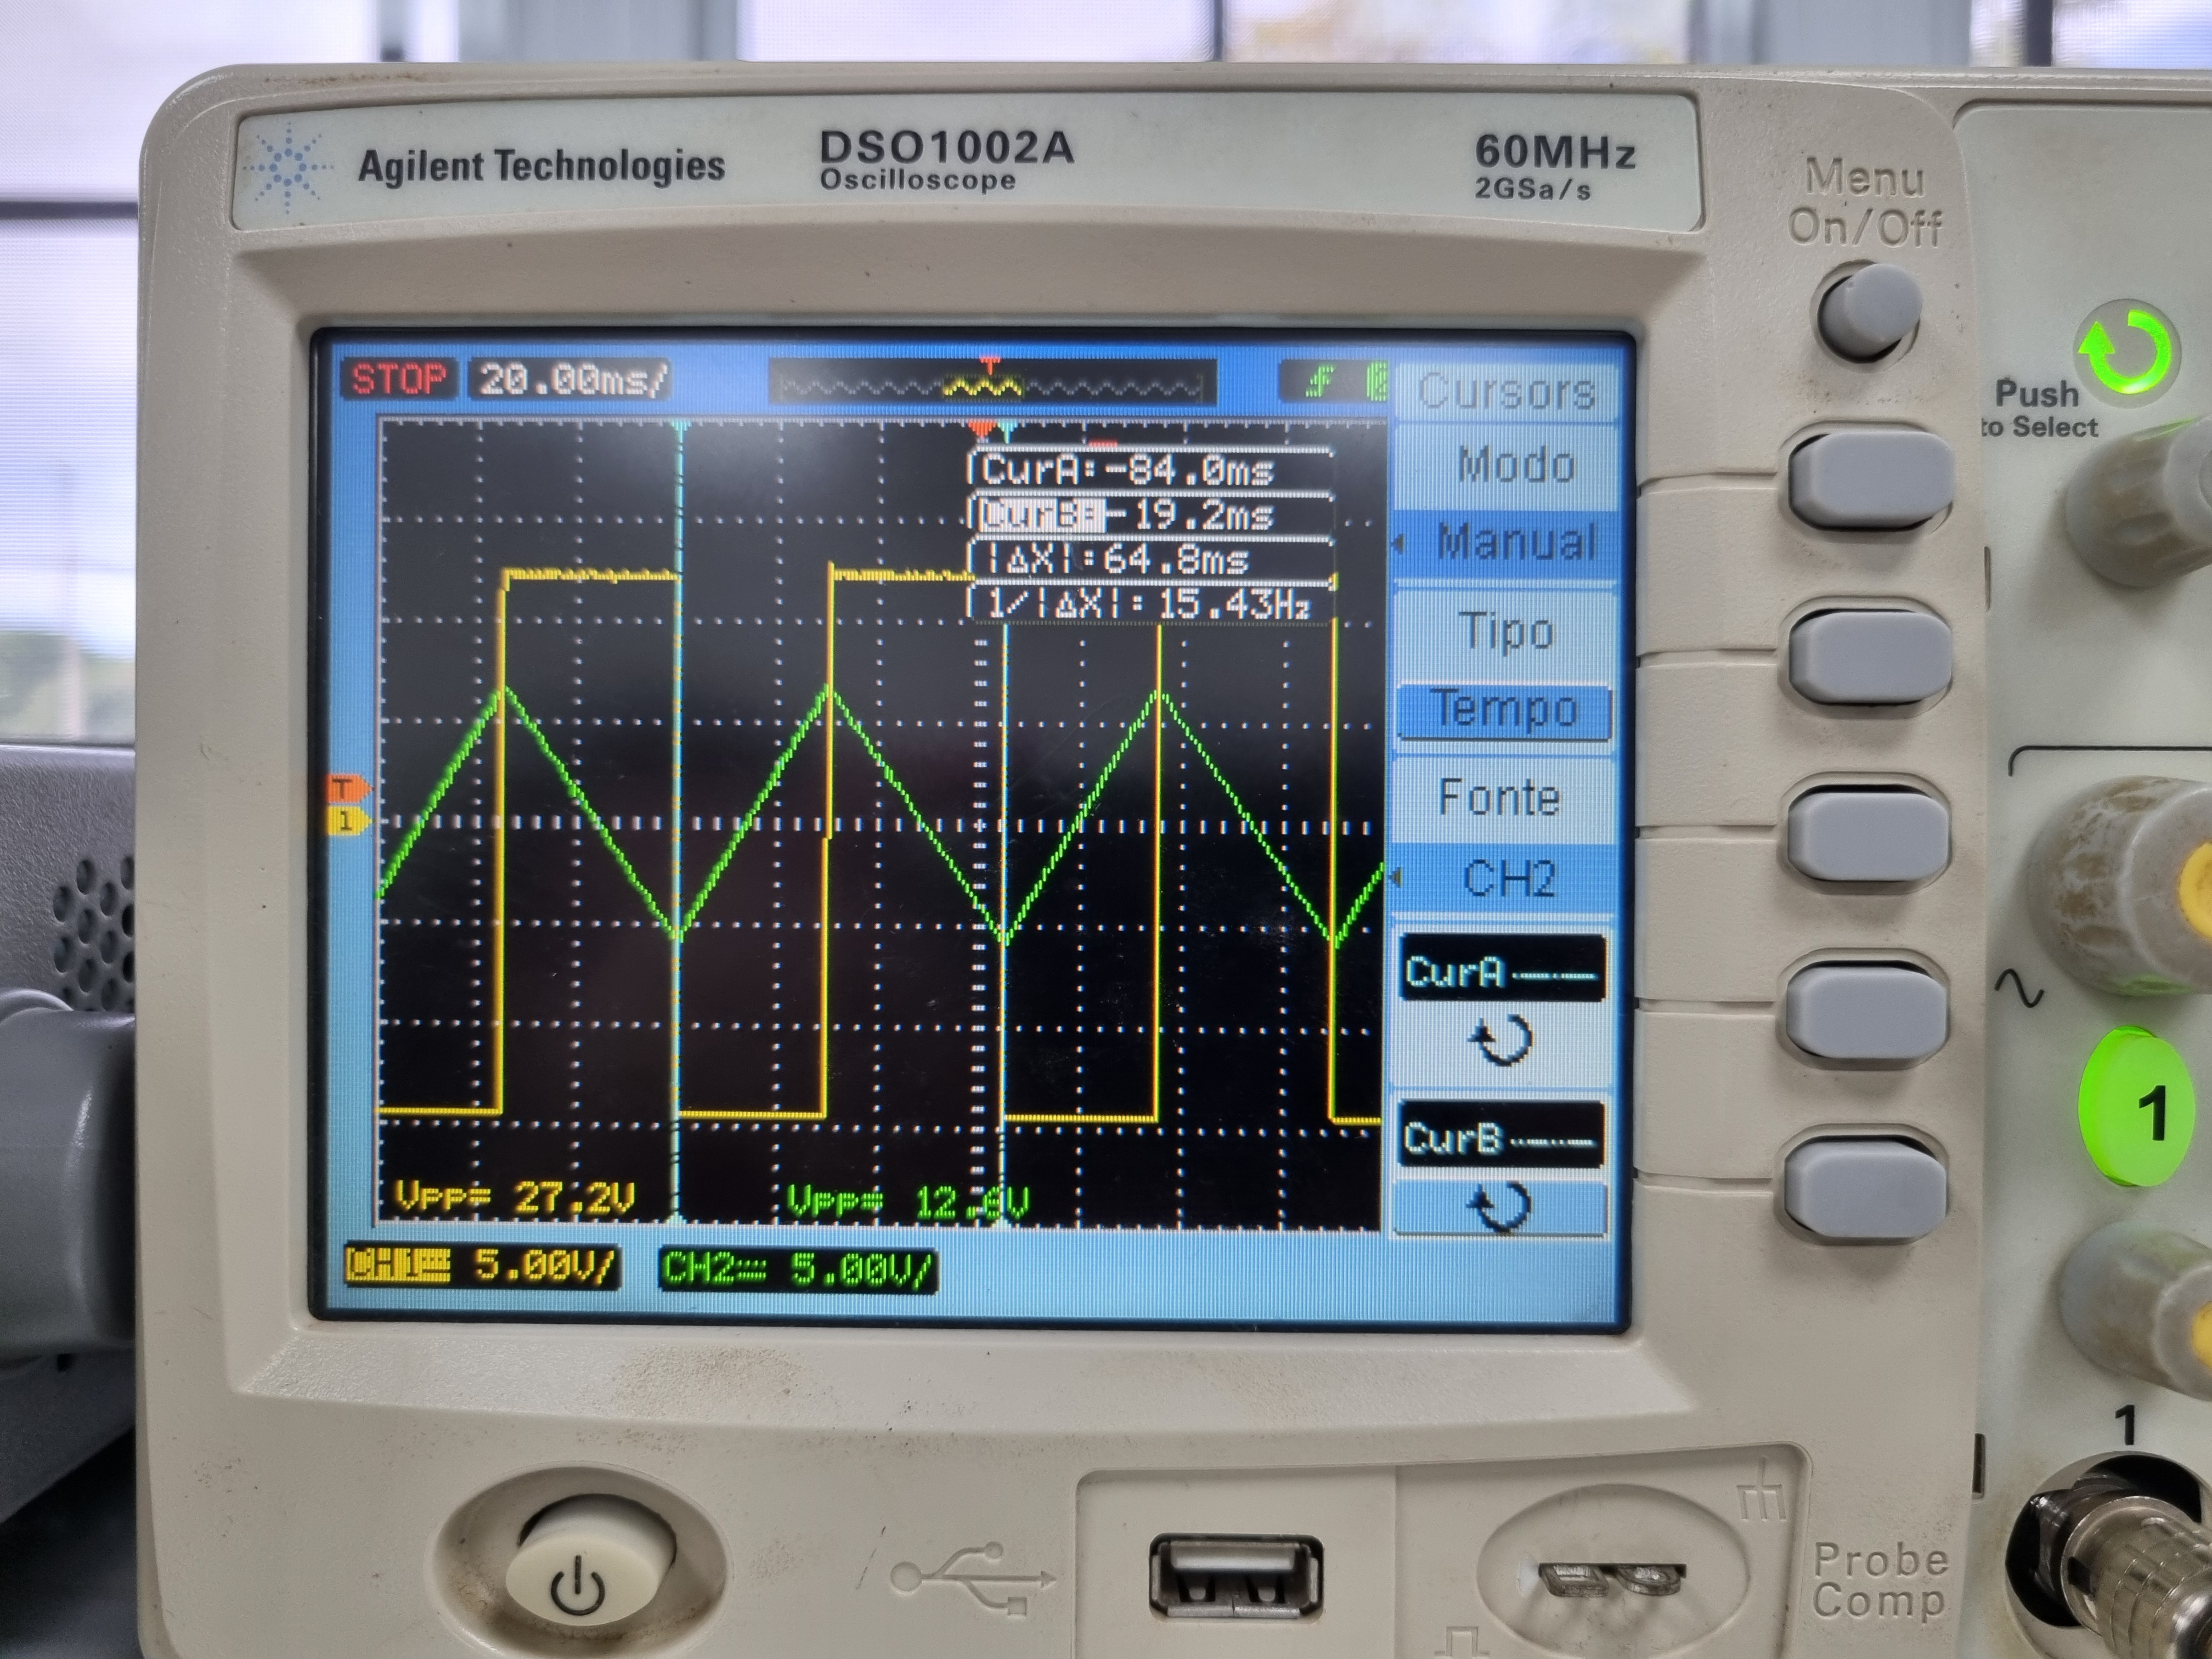
\includegraphics[width=0.8\linewidth]{imagens/ocl_frequencia_gerador.jpg}
	\caption{Frequências da saida do gerador medida com cursores. Foi obtido o valor de \SI{15.43}{\hertz}}
  \label{fig:ocl_frequencia_gerador.jpg}
\end{figure}

\begin{center}
  \begin{tabular}{@{}lrrrr@{}}
    \toprule
    \textbf{Grandeza} & \textbf{Projeto} & \textbf{Sim. montagem} & \textbf{Medido} &
    \textbf{Erro} \\
    \midrule
    Frequência & \SI{}{\hertz} & \SI{23.4}{\hertz} & \SI{15.43}{\hertz} & \\
    \bottomrule
  \end{tabular}
\end{center}

\subsubsection{Amplificador e conformador}

\begin{center}
  \begin{tabular}{@{}lrrrr@{}}
    \toprule
    \textbf{Grandeza} & \textbf{Projeto} & \textbf{Sim. montagem} & \textbf{Medido} &
    \textbf{Erro} \\
    \midrule
    Tensão $V_1$ & \SI{4,6}{\volt} & \SI{3.9}{\volt} & \SI{3.9}{\volt} & \\
    Tensão $V_2$ & \SI{7,2}{\volt} & \SI{6.5}{\volt} & \SI{6.5}{\volt} & \\
    Tensão $V_3$ & \SI{8,9}{\volt} & \SI{8.2}{\volt} & \SI{8.2}{\volt} & \\
    \bottomrule
  \end{tabular}
\end{center}

\begin{figure}[H]
  \centering
  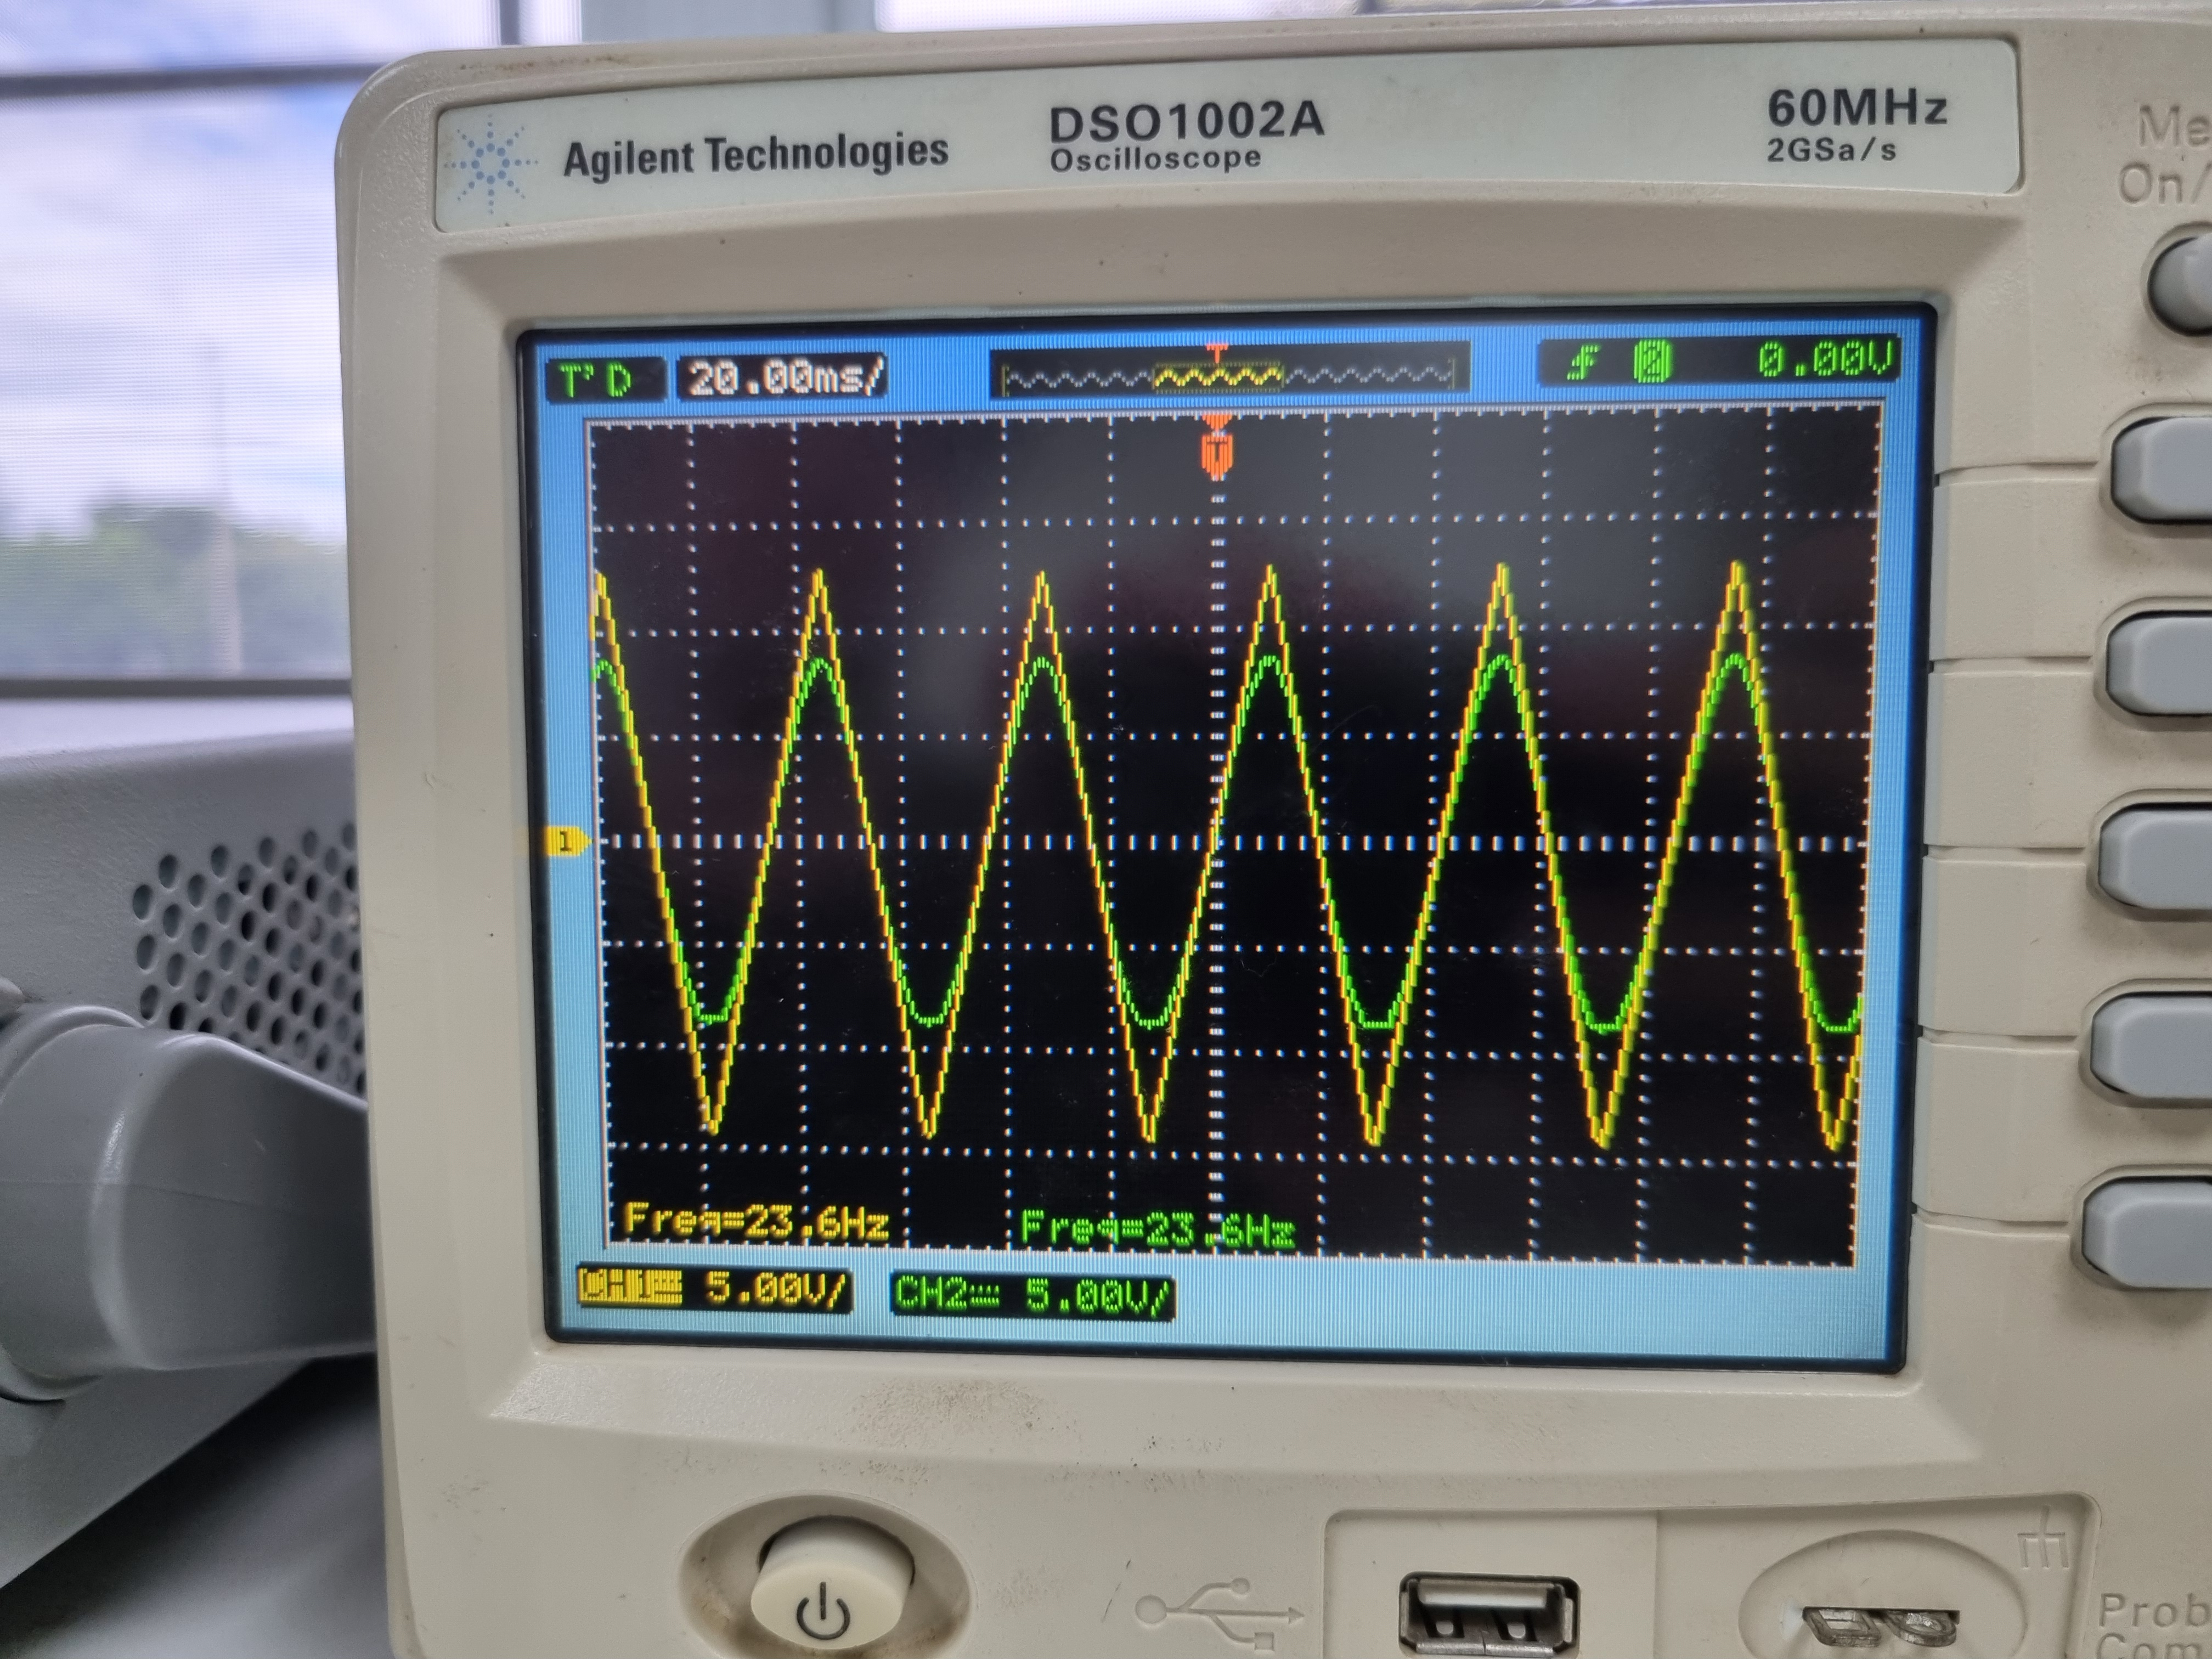
\includegraphics[width=0.8\linewidth]{imagens/ocl_conformador.jpg}
  \caption{imagem ocl saida conformador.jpg}
  \label{fig:ocl_saida_conformador.jpg}
\end{figure}

\section{Discussão}

Percorra as três comparações na ordem em que aparecem no quadro da Seção~4: a conta contra
a simulação de projeto, esta contra a simulação da montagem, e esta contra a medição. Cada
passo isola uma causa, e a discussão fica bem mais curta quando eles não se misturam.

Compare também os projetos dos integrantes entre si. Como as especificações são diferentes,
os resultados diferem, e mostrar que essa diferença é a que a teoria previa vale mais do
que repetir três vezes a mesma análise.

Sempre que uma divergência for maior do que a incerteza esperada, aponte uma causa concreta
e diga como ela poderia ser reduzida. Vale, por exemplo, a tolerância do componente, a
resistência série do indutor, a impedância de entrada do osciloscópio, a banda do
amplificador ou a resolução da varredura.

Quando previsto e obtido coincidirem, explique por que era esperado que coincidissem, e o
que essa coincidência não permite concluir.

Por fim, retome as hipóteses que vocês declararam na fundamentação e diga quais se
confirmaram. Se algo observado contrariar a previsão, resolva a contradição aqui.

\section{Conclusão}

Retome o objetivo que vocês anunciaram na introdução e responda se ele foi atingido,
apoiando a resposta em um número. Aponte a principal limitação do que foi feito e o que
ela impede de afirmar. Evite trazer resultado novo nesta seção.

\section{Referências}

\begin{referencias}
\item SEDRA, A.~S.; SMITH, K.~C. \emph{Microeletrônica}. 5.~ed. São Paulo: Pearson
  Prentice Hall, 2007.
\item BOYLESTAD, R.~L.; NASHELSKY, L. \emph{Dispositivos Eletrônicos e Teoria de
  Circuitos}. 11.~ed. São Paulo: Pearson Education do Brasil, 2013.
\end{referencias}

\end{document}
